\chapter{Information Flow Analysis using Denning's Lattice Model}
\label{ch:denning}
\section{Analysis In Local Scope}
We started certification of python code at local scope initially.
\begin{figure}[ht]
	
	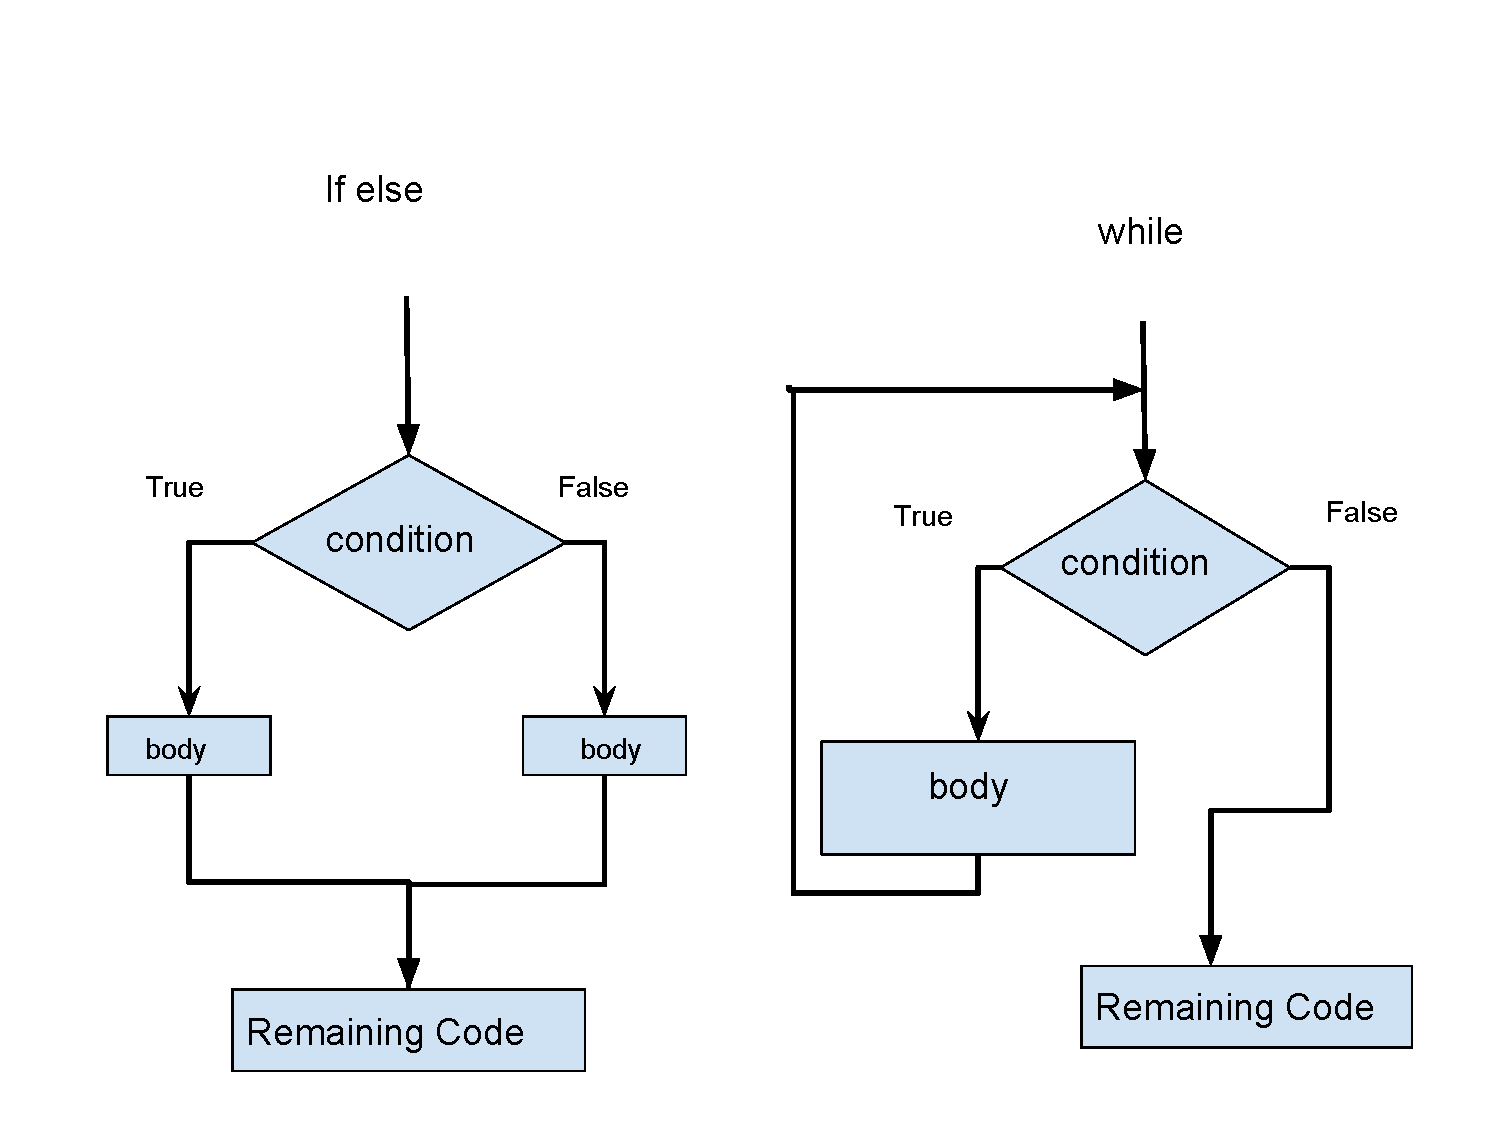
\includegraphics[width=0.8\textwidth]{branching}
	\caption{Control flow graph of If else and while loop}
	\label{fig:branching}
\end{figure}
In figure \ref{fig:branching} we considered information flowing from variables used in condition to targets of assignment operation in body code only. Further analysis will be dealing with information flows to targets of assignment in remaining code. Now a program with if else and terminating loops can be certified to be secure (no information leaks) by using basic rules of information theory implemented in my script.\\
\textit{Fifth chapter of Denning's book\cite{denning} used six examples to describe how can information flow through different ways in the program. We used python version of these examples as benchmark.}\\
\subsection{Benchmarking of Certification Script using Denning's Examples \cite{denning}}
\begin{lstlisting}[language=Python, caption=Python version of copy1 example in \cite{denning}. goal: information flow from x to y, label={lst:copy1} ]
#Procedure copy1
x = 0
z = 0
y = 0
if x == 0:
	z=1
if z == 0:
	y=1
\end{lstlisting}
Constraints for program in \ref{lst:copy1} generated by our script are:\\
\begin{enumerate}
	\item low $\leqslant$ \dud{x}
	\item low $\leqslant$ \dud{z}
	\item low $\leqslant$ \dud{y}
	\item low $\leqslant$ \dud{y}
	\item \dud{x} $\leqslant$ \dud{z}
	\item \dud{z} $\leqslant$ \dud{y}
\end{enumerate}
Program in listing \ref{lst:copy1} shows how  information can flow indirectly from x to y, for secure information flow $ \dud{x} \leqslant \dud{y} $ must be true. Constraint 5 (x $\leqslant$ z) and constraint 6 (z $\leqslant$ y) with transitivity property of lattice model satisfies x $\leqslant$ y.  \\
\begin{lstlisting}[language=Python, caption=Python version of copy2 example in \cite{denning}. goal: information flow from x to y, label={lst:copy2} ]
# Procedure copy2
x = 0
z = 1
y = -1
while z == 1:
	y = y + 1
	if y == 0:
		z = x
	else:
		z = 0
\end{lstlisting}
Constraints of program in Listing \ref{lst:copy2} generated by our script are:\\
\begin{enumerate}
\item low $\leqslant$ \dud{x}
\item low $\leqslant$ \dud{z}
\item low $\leqslant$ \dud{y}
\item \dud{y} $\oplus$ \dud{z} $\leqslant$ \dud{y}
\item \dud{y} $\oplus$ \dud{x} $\oplus$ \dud{z} $\leqslant$ \dud{z}	
\end{enumerate}
Information flows from x to y using iteration of the while loop in listing \ref{lst:copy2}.
One iteration of while loop changes the value of y to -1 to 0 by incrementing it by 1, and two iteration of same while loop changes the value of y to -1 to 1. Number of iterations of while loop depends on value of x so this program is transmitting information from x to y indirectly using both explicit and implicit information flows.\\  
\textbf{\textit{Proof:}}\\
\dud{x} $\leqslant$ \dud{y} must be true for secure information flow. This can be proved using constraint 4 ( \dud{y} $\oplus$ \dud{z} $\leqslant$ \dud{y})
and constraint 5 (\dud{y} $\oplus$ \dud{x} $\oplus$ \dud{z} $\leqslant$ \dud{z}) in two ways. First: \dud{z} $\leqslant$ \dud{y} is given in constraint 4 and \dud{y} $\leqslant$ \dud{z} is given in constraint 5 so \dud{y} must be equal to \dud{z} using this new constraint ( \dud{y} $\equiv$ \dud{z} ) and reduced constraint 5 (\dud{x} $\leqslant$ \dud{z}) desired constraint \dud{x} $\leqslant$ \dud{y} is proved.  
\section{Further analysis: considering global influence of while}
A program either terminates after a finite period of time or executes for an infinite period of time. The latter can be achieved through while loop and for loop. Such a non-terminating loop influences variables within the body of the loop as well as after the body of loop.
 \begin{lstlisting}[language=Python, caption=Non terminating while., label={lst:ntwhile} ]
 x = 0
 z = True
 y = 0
 while z :
	 y = 5
x = 5	
 \end{lstlisting}
In listing \ref{lst:ntwhile} execution of last statement x = 5 is conditioned on "while z" statement similar to "if" branching but "if" has limited body but in this case every statement that comes after "while z" share fate with x = 5, because of this property of "while" it is very crucial to know whether loop is terminating or nonterminating, so either there should be a mechanism to determine to terminating and nonterminating nature of loop or treat all while loop as nonterminating, latter approach is imprecise but secure, for now we are using this approach to handle while loops.
\subsection{Benchmarking of Certification Script using Denning's Examples \cite{denning}}
\begin{lstlisting}[language=Python, caption=Python version of copy5 example in \cite{denning}. goal: information flow from x to y, label={lst:copy5} ]
#Procedure copy5
y = 0
while x==0 :
	pass
y = 1
\end{lstlisting}  
Constraints generated by our script:
\begin{enumerate}
	\item low $\leqslant$ \dud{y}
	\item \dud{x} $\leqslant$ \dud{y}
\end{enumerate}
so here our script able to track information flow from x to y and generating constraint \dud{x} $\leqslant$ \dud{y} for verification.

\begin{lstlisting}[language=Python, caption=Python version of copy4 example in \cite{denning}. goal: information flow from x to y, label={lst:copy4} ]
#Procedure copy4
import thread
import time
import threading

def thread1():
global x
global e0
global e1
if x==0:
	e0 = False
else:
	e1 = False

def thread2(): 
global e0
global e1
global y
while e0
	pass
y = 1
e1 = False

def thread3():
global e1
global e0
global y
while e1:
	pass
y = 0
e0 = False

thread.start_new_thread(thread1,())
thread.start_new_thread(thread2,())
thread.start_new_thread(thread3,())\end{lstlisting}

Constraints generated by our script for program in listing \ref{lst:copy4} are:
\begin{enumerate}
	\item \dud{x} $\leqslant$ \dud{e0}
	\item \dud{x} $\leqslant$ \dud{e1}
	\item \dud{e0} $\leqslant$ \dud{y}
	\item \dud{e0} $\leqslant$ \dud{e1}
	\item \dud{e1} $\leqslant$ \dud{y}
	\item \dud{e1} $\leqslant$ \dud{e0}
\end{enumerate}
(\dud{x} $\leqslant$ \dud{e0} ) and (\dud{e0} $\leqslant$ \dud{y}) \hspace{1cm} $\equiv$ \hspace{1cm} \dud{x} $\leqslant$ \dud{y} (transitivity)\\
(\dud{x} $\leqslant$ \dud{e1} ) and (\dud{e1} $\leqslant$ \dud{y}) \hspace{1cm} $\equiv$ \hspace{1cm} \dud{x} $\leqslant$ \dud{y}\\
So script able to track hidden information flow from x to y and generating constraint for this flow \dud{x} $\leqslant$ \dud{y} by using transitivity.
